\documentclass[aspectratio=169]{beamer}
\usepackage[english]{babel}
\usepackage{booktabs,listings}
\usepackage[T1]{fontenc}
\usepackage[utf8]{inputenc}
\usepackage{xcolor}
\usepackage{graphicx}
\usepackage{upgreek}
\usepackage{amsmath}
\usepackage{amssymb}
\usepackage{amsbsy}
\usepackage{tikz}
\usepackage[american]{circuitikz}
\usetikzlibrary{fit}
\usetikzlibrary{circuits.ee.IEC}
\lstset{basicstyle=\ttfamily}
\setlength{\parskip}{.5\baselineskip}
\usetheme[style=vertical, frametotal=true]{NTNU}
%define new color name NTNU_blue with rgb value 124,137,52
\definecolor{NTNU_blue}{RGB}{96,150,208} % blue
\definecolor{NTNU_green}{RGB}{188,208,37} % green
\definecolor{NTNU_orange}{RGB}{239,129,20} % orange
\definecolor{NTNU_purple}{RGB}{72,39,118} % purple
\definecolor{NTNU_sand}{RGB}{207,184,135}

\usetikzlibrary{positioning,calc}

\usepackage[backend=biber,style=numeric,sorting=none]{biblatex}
\addbibresource{reference.bib}


\title{Current Physical Component (CPC) power theory}
\subtitle{Course ET8304}
\author{Andreetta Niccolò}
\date{April $12^{th}$, 2024}

\begin{document}
  \maketitle

  \begin{frame}[fragile]{Outline}
    \tableofcontents
  \end{frame}

  \section{Introduction}
  \begin{frame}{Evolution and philosophy}{\insertsection}
        CPC power theory started to be developed in \textcolor{NTNU_orange}{1984} by Leszek S. Czarnecki.\\
        Most cited article according to Scholar is \textit{"What is wrong with the Budeanu concept of reactive and distortion power and why it should be abandoned"} \cite{6312797}.
        \begin{itemize}
            \item Currents are not related with physical phenomenon in the circuit
            \item Currents are useless for compensator's design
            \item Distortion power does not provide information about waveform distortion
        \end{itemize}
        \textcolor{NTNU_orange}{Increasing complexity}: initially for single phase circuits with LTI loads supplied with non-sinusoidal voltages, and then the extensions.\\
        
  \end{frame}

  \begin{frame}[fragile]{Motivation}{\insertsection}        
    \begin{figure}
      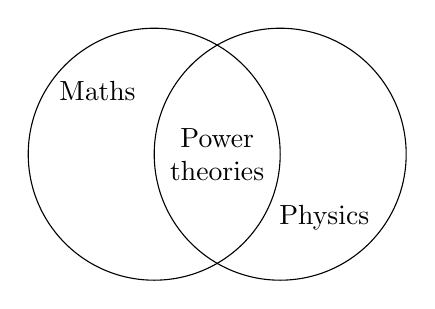
\begin{tikzpicture}[scale=0.8]
        % Left circle (Mathematics)
        \draw (0,0) circle (2cm);
        \node at (-0.9,1) {Maths};
        
        % Right circle (Physics)
        \draw (2,0) circle (2cm);
        \node at (2.7,-1) {Physics};
        
        % Intersection
        \node[align=center] at (1,0) {Power \\ theories};
        
      \end{tikzpicture}
    \end{figure}

      Not all the the power theories are correct from the physical point of view, even tough they are mathematically correct.\\

      \textbf{Physical} does not mean that the current exists physically, but they are associated with some physical phenomenon in the load. 
      
  \end{frame}

\section{1 phase circuits with LTI loads}
  \begin{frame}{1 phase circuits with LTI loads}
  Given the supply voltage $u(t)$ and the harmonic dependent load admittance $Y_n$
    \begin{gather}
      u(t) = U_0 + \sqrt{2}Re\left\{\sum_{n\in N}U_n e^{jn\omega_1t}\right\}\\
      Y_n = G_n + jB_n
    \end{gather}

    \begin{figure}
      \centering
      \begin{circuitikz}[scale=0.7]
        \draw (0,0) to [nV, l=$u(t)$] (0,2) to [short,i=$i(t)$] (4,2) to [generic, l=$Y_n$] (4,0) to [short] (0,0);
      \end{circuitikz}
    \end{figure}

The current is
    \begin{equation}
      i(t) = Y_0U_0 + \sqrt{2}Re\left\{\sum_{n\in N}Y_n U_n e^{jn\omega_1t}\right\}
    \end{equation}
  \end{frame}

  \begin{frame}{Active current}{\insertsection}
    \begin{equation}
      i(t) = Y_0U_0 + \sqrt{2}Re\left\{\sum_{n\in N}Y_n U_n e^{jn\omega_1t}\right\}
    \end{equation}

  We can assume there is an \textcolor{NTNU_orange}{Active current}: the current of a resistive equivalent load that at the same voltage $u(t)$ has the same active power P as the original load
  \begin{equation}
    i_a(t) = G_e u(t) = G_e U_0 + \sqrt{2}Re\left\{\sum_{n\in N}G_e U_n e^{jn\omega_1t}\right\} 
  \end{equation}
  with \textcolor{NTNU_orange}{equivalent conductance} $G_e = \frac{P}{||u||^2}$.

  \end{frame}

  \begin{frame}{Reactive and scattered currents}{\insertsection}
  The remaining current is:
  \begin{gather}
    i(t)-i_a(t) = (Y_0-G_e)U_0 + \sqrt{2}Re\left\{\sum_{n\in N}(Y_n-G_e)U_n e^{jn\omega_1t}\right\}=\notag \\
    (Y_0-G_e)U_0 + \sqrt{2}Re\left\{\sum_{n\in N}(G_n+jB_n-G_e)U_n e^{jn\omega_1t}\right\}
  \end{gather}
  And can be decomposed in \textcolor{NTNU_orange}{Reactive current} $i_r(t)$ and  \textcolor{NTNU_blue}{Scatter current} $i_s(t)$
  \begin{gather}
    \textcolor{NTNU_orange}{i_r(t)} = \sqrt{2} Re\left\{\sum_{n\in N}j B_n U_n e^{jn\omega_1t}\right\}\\
    \textcolor{NTNU_blue}{i_s(t)} = (G_0-G_e)U_0 + \sqrt{2}Re\left\{\sum_{n\in N}(G_n-G_e)U_n e^{jn\omega_1t}\right\}
  \end{gather}

  \end{frame}

  \begin{frame}{Physical interpretation}{\insertsection}
  The supply current can be expressed as:
    \begin{equation}
      i(t) = i_a(t) + i_r(t) + i_s(t)
    \end{equation}

    Physical meaning:
    \begin{itemize}
      \item \textbf{Active current}: permanent energy conversion
      \item \textbf{Scattered current}: change of the $G_n$ with harmonic order
      \item \textbf{Reactive current}: phase shift between the voltage and current harmonics
    \end{itemize}

    \textbf{\textcolor{NTNU_blue}{Physical}} does not mean that the current exists physically, but they are associated with some physical phenomenon in the load. 
  \end{frame}

  \begin{frame}{RMS values of the currents}{\insertsection}
  The RMS of the currents:
      \begin{gather}
            ||i_a||=G_e||u||=\frac{P}{||u||}\\
            ||i_s||=\sqrt{\sum_{n \in N_0}(G_n-G_e)^2U_n^2}\\
            ||i_r||=\sqrt{\sum_{n\in N}B_n^2U_n^2}=\sqrt{\sum_{n\in N}\left(\frac{Q_n}{U_n}\right)^2}
      \end{gather}
      For compute the RMS of the load current having RMSs of the component, their orthogonality is required, and following prove.
  \end{frame}

  \begin{frame}{Orthogonality of the currents}{\insertsection}
    Remark scalar product: $(a,b) = \frac{1}{T}\int_{0}^{T}a(t)b(t)dt=Re\left\{\sum_{n\in N_0}A_nB_n^*\right\}$
  
    \begin{gather}
      (i_r, i_a) = Re\left\{\sum_{n \in N}jB_eU_nG_eU_n^*\right\} =  Re\left\{\sum_{n \in N}jB_eG_eU_n^2\right\} = 0\\
      (i_s, i_a) = Re\left\{\sum_{n \in N}(G_n-G_e)U_nG_eU_n^*\right\} = G_e Re\left\{\sum_{n \in N}(G_n-G_e)U_n^2\right\} = \notag\\
      = G_e\left( \sum_{n\in N}G_nU_n^2-G_e\sum_{n\in N}U_n^2\right) = G_e\left(P-G_e||u||^2\right)=0\\
      (i_r, i_s) = Re\left\{\sum_{n\in N}jB_eU_n(G_n-G_e)U_n^*\right\}=0
    \end{gather}
    Orthogonality is proved
  \end{frame}
      
  \begin{frame}{Orthogonality of the currents-cont.}{\insertsection}
    So the current can be expressed as:
    \begin{equation}
      ||i||^2 = ||i_a||^2 + ||i_r||^2 + ||i_s||^2
    \end{equation}

    \begin{figure}
      \centering
      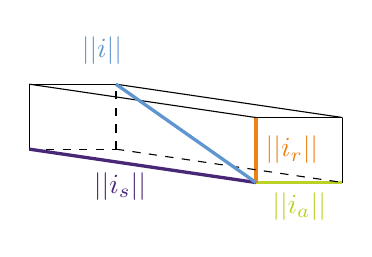
\begin{tikzpicture}[scale=1.1]
        % Cube vertices
        \coordinate (A) at (0,0,0);
        \coordinate (B) at (1,0,0);
        \coordinate (C) at (1,0.75,0);
        \coordinate (D) at (0,0.75,0);
        \coordinate (E) at (3,0,1);
        \coordinate (F) at (4,0,1);
        \coordinate (G) at (4,0.75,1);
        \coordinate (H) at (3,0.75,1);
        % Draw edges
        \draw[dashed] (A) -- (B);
        \draw[dashed] (B) -- (C);
        \draw (C) -- (D);
        \draw (D) -- (A);
        \draw[line width=1.2pt, NTNU_green] (E) -- (F);
        \draw (F) -- (G);
        \draw (G) -- (H);
        \draw[line width=1.2pt, NTNU_orange] (H) -- (E);
        \draw[line width = 1.2pt, NTNU_purple] (A) -- (E);
        \draw[dashed] (B) -- (F);
        \draw (C) -- (G);
        \draw (D) -- (H);
        \draw[line width=1.2pt, NTNU_blue] (E) -- (C);
        % Label edges
        \node[below, NTNU_green] at ($(E)!0.5!(F)$) {$||i_a||$};
        \node[below, NTNU_purple] at ($(E)!0.6!(A)$) {$||i_s||$};
        \node[right, NTNU_orange] at ($(E)!0.5!(H)$) {$||i_r||$};
        \node[above, NTNU_blue] at ($(E)!1.1!(C)$){$||i||$};
        \end{tikzpicture}
    \end{figure}
    
    An the power as:
    \begin{gather}
      \textcolor{NTNU_blue}{||i||^2||u||^2} =  \textcolor{NTNU_green}{||i_a||^2||u||^2} + \textcolor{NTNU_orange}{||i_r||^2||u||^2}  + \textcolor{NTNU_purple}{||i_s||^2||u||^2}\\
      \textcolor{NTNU_blue}{S^2} = \textcolor{NTNU_green}{P^2} + \textcolor{NTNU_orange}{Q^2} + \textcolor{NTNU_purple}{D_s^2}
    \end{gather}

    \textcolor{NTNU_purple}{$D_s$} Scattered and \textcolor{NTNU_orange}{$Q$} Reactive  (NOTE: Different from Budeanu's)

  \end{frame}

  \begin{frame}{Compensation}{{\insertsection}}
    Traditionally compensators were used to reduce the reactive current RMS value, while nowadays they have to compensate also load imbalance or power variations. \\
    \textcolor{NTNU_orange}{Can the PF of a load under non-sinusoidal conditions be improved by a reactance compensator?} \textcolor{NTNU_purple}{(Spoiler: YES)}
  \end{frame}

  \begin{frame}{Compensation-cont.}{\insertsection}
  Take a reactance compensator ($Y_{Cn}=jB_{Cns}$) not affecting: U, P, $D_s$
   \begin{figure}
    \centering
    \begin{circuitikz}[scale=1]
      \draw (0,0) to[open, v=$u(t)$, voltage=straight, o-o] (0,2);
        \draw (0,2) to[short, i=$i_a+i_s+i_r'$] (2,2);
        \draw (0,0) to[short] (4,0);
        \draw (2,0) to[generic=$LC$] (2,2);
        \draw (2,2) to[short, i=$i_a+i_s+i_r$] (4,2);
        \draw (4,0) to[generic=$LTI$] (4,2);      
    \end{circuitikz}
    \end{figure}

    The reactive current is modified as:
    \begin{equation}
        i_r' = \sqrt{2}Re\left\{\sum_{n\in N}j(B_n+B_{Cn})U_ne^{jn\omega_1t}\right\}
    \end{equation}
    total compensation when $B_{Cn}=-B_n$. The max PF becomes:
    \begin{equation}
        \lambda=\lambda_{MAX}=\frac{P}{S}=\frac{||i_a||}{\sqrt{||i_a||^2+||i_s||^2}}
    \end{equation}
  \end{frame}

\section{1 phase circuits with HGL}
\begin{frame}{Introduction example}{\insertsection}
  Now take into account Harmonic Generating Load (HGL). \\
   As example assume:
    \begin{itemize}
      \item Supply voltage of $e=e_1=100\sqrt{2}sin(\omega_1 t)$ \
      \item The load generates a third order harmonic $j=j_3=50\sqrt{2}sin(3\omega_1t)$
    \end{itemize}

    \begin{figure}
    \centering
    \begin{circuitikz}[scale=1]
      % Voltage source on the left
      \draw (0,0) to [nV, l=$e(t)$] (0,2)
      % 1 ohm resistor
      (0,2) to [generic=$1\Omega$] (2,2)
      (2,2) to [short, -o] (3,2)
      % Connection to shunt resistor and current source
      to [short] (4,2)
      to [generic=$4\Omega$] (4,0)
      -- (0,0);
      \draw (4,2) to [short, f=$i(t)$] (5.5,2);
      \ctikzset{bipoles/noise sources/fillcolor=dashed}
      \begin{scope}
          \draw (5.5,2) to [nI, l=$j$, fill=white] (5.5,0); 
      \end{scope}
      \draw (5.5,0) to [short, -o] (3,0);
      % Voltage measurer         
      \draw (3,2) to[open, v<=$u(t)$, voltage=straight, o-o] (3,0);
      
      % Draw square and label
      \node[draw, dashed, fit={(-0.85,0) (1.5,2.5)}, inner sep=12pt, label=above:Supply] {};
      \node[draw, dashed, fit={(4,0) (6,2.5)}, inner sep=10pt, label=above:HGL] {};
    \end{circuitikz}
    \end{figure}
\end{frame}

\begin{frame}{Introduction example-cont.}{\insertsection}
    The voltage and currents at load terminals are:
    \begin{gather}
      u=u_1+u_3 = 80\sqrt{2}sin(\omega_1t)-40\sqrt{3\omega_1t} \ \left[V\right]\\
      i=i_1+i_3 = 20\sqrt{2}sin(\omega_1t)+40\sqrt{3\omega_1t} \ \left[A\right]
    \end{gather}
    thus the powers are 
    \begin{gather}
      P=\sum_{n=1,3}U_nI_n cos(\varphi_n)=1600-1600=0 \ \left[W\right]\\
      S = ||u||||i|| = 4000 \ \left[VA\right]\\
      S \ne P^2+Q^2+D_s^2;
    \end{gather}
    The reason is the presence of P associated with the $3^{rd}$ order harmonic of value $P=-1600\ \left[W\right]$. This P is generated by the load and dissipated in the supply source resistance. \textcolor{NTNU_orange}{There is a current component in the supply current which cannot be interpreted as $i_r$ or $i_s$ but it does not contribute to the load active power.}
  \end{frame}

  \begin{frame}{Sign of the power}{\insertsection}
    \textcolor{NTNU_orange}{The presence of current harmonic generated in the load has to be considered as a phenomenon that affects the power properties of the circuits.}\\
    Possibly bi-directional power flow:
    \begin{equation}
      P_n = U_nI_n cos(\varphi_n)
    \end{equation}
    \begin{itemize}
      \item $|\varphi_n|<\pi/2 \Rightarrow$ energy flow from \textcolor{NTNU_purple}{supply source} towards the \textcolor{NTNU_green}{load}
      \item $|\varphi_n| >\pi/2 \Rightarrow$ energy flow  from \textcolor{NTNU_green}{load} towards the \textcolor{NTNU_purple}{supply source}
    \end{itemize}
\end{frame}

\begin{frame}{Harmonics division}{\insertsection}
    Then we can divide the harmonics in two sets:
    \begin{itemize}
      \item $|\varphi_n|<\pi/2 \Rightarrow n\in N_D$ 
      \item $|\varphi_n| >\pi/2 \Rightarrow n\in N_C$ 
    \end{itemize}
    \begin{gather}
      i=\sum_{n\in N}i_n = \sum_{n \in N_D}i_n + \sum_{n \in N_C}i_n = i_D+i_C\\
      u=\sum_{n\in N}u_n = \sum_{n \in N_D}u_n + \sum_{n \in N_C}u_n = u_D \textcolor{red}{-}u_C\\
      P=\sum_{n\in N}P_n = \sum_{n \in N_D}P_n + \sum_{n \in N_C}P_n = P_D - P_C
    \end{gather}
    Change of sign in $u_C$ because is a voltage produced by the load.\\
    $N_C$ and $N_D$ don't contain common harmonics $\Rightarrow$ Orthogonal: 
    \begin{gather}
        ||i||^2=||i_D||^2+||i_C||^2\\
        ||u||^2=||u_D||^2+||u_C||^2\\
    \end{gather}
  \end{frame}
  
  \begin{frame}{Superimposition principle}{\insertsection}
  Orthogonality $\Rightarrow$ Superimposition principle
    \begin{figure}
      \centering
      \begin{circuitikz}[scale = 0.8]
        % Voltage source on the left
        \draw (0,0) to [nV, l=$e_D$] (0,2)
        % 1 ohm resistor
        (0,2) to [generic] (2,2)
        (2,2) to [short, -o] (3,2)
        % Connection to shunt resistor and current source
        to [short] (4,2);
        \draw (5.5,0) to [short, -o] (3,0);
        % to [short] (4,0);
        % -- (0,0);
        \draw (4,2) to [short, f=$i_D$] (5.5,2);
        \draw (5.5,2) to [generic=$Y$] (5.5,0); 
        % Voltage measurer         
        \draw (3,2) to[open, v<=$u_D$, voltage=straight, o-o] (3,0);
        \draw (0,0) to [short] (3,0);
        % Draw square and label
        \node[draw, dashed, fit={(-0.85,0) (1.5,2.5)}, inner sep=8pt, label=above:Supply] {};
        \node[draw, dashed, fit={(4,0) (6,2.5)}, inner sep=8pt, label=above:HGL] {};
      \end{circuitikz}
  
      \begin{circuitikz}[scale=0.8]
        % Voltage source on the left
        \draw (0,0) to [short] (0,2)
        % 1 ohm resistor
        (0,2) to [generic] (2,2)
        (2,2) to [short, -o] (3,2)
        % Connection to shunt resistor and current source
        to [short] (4,2);
        % to [generic=$4\Omega$] (4,0)
        \draw (3,0) to [short] (0,0);
        \draw (4,2) to [short, f=$i_C$] (5.5,2);
        \ctikzset{bipoles/noise sources/fillcolor=dashed}
        \begin{scope}
            \draw (5.5,2) to [nI, l=$j_C$, fill=white] (5.5,0); 
        \end{scope}
        \draw (5.5,0) to [short, -o] (3,0);
        % Voltage measurer         
        \draw (3,2) to[open, v<=$u_C$, voltage=straight, o-o] (3,0);
        
        % Draw square and label
        \node[draw, dashed, fit={(0,0) (1.5,2.5)}, inner sep=8pt, label=above:Supply] {};
        \node[draw, dashed, fit={(4,0) (6.25,2.5)}, inner sep=8pt, label=above:HGL] {};
      \end{circuitikz}
      
      \end{figure}

  \end{frame}

  \begin{frame}{Orthogonality of the currents}{\insertsection}
    The \textit{D circuit} can be analyzed as before, and the $i_D$ decomposed as:
    \begin{equation}
      i_D = i_a + i_s + i_r
    \end{equation}
    then it can be back substituted and 
    \begin{gather}
      i = i_D+i_C = i_a + i_s + i_r + i_C\\
      ||i||^2 = ||i_a||^2 + ||i_s||^2 + ||i_r||^2 + ||i_C||^2
    \end{gather}

    \begin{figure}
      \centering
      \scalebox{0.9}{\input{current_schema.pdf_tex}}
      \end{figure}
  \end{frame}

\section{3 phase systems with sinusoidal voltages and currents}
  \begin{frame}{Non-univocal definition of S}{\insertsection}
    Confusion in the definition of the Apparent Power since three definitions coexist:
    \begin{gather}
    S_A = U_RI_R+U_SI_S+U_TI_T\\
    S_G = \sqrt{P^2+Q^2}\\
    S_B = \sqrt{U_R^2+U_S^2+U_T^2}\sqrt{I_R^2+I_S^2+I_T^2}  
    \end{gather}
    These are the same only if line currents are sinusoidal and symmetrical. The power factor behaves consequently. 
  \end{frame}

  \begin{frame}{Reference circuit and notation}{\insertsection}
  Consider a 3 phase 3 wire system connected to a $\Delta$ load
    \begin{figure}
    \centering
    \begin{circuitikz}[scale = 0.5]
      \draw (0,3) node[ocirc, label=R]{} to (3,3);
      \draw (0,0) node[ocirc, label=S]{} to (3,0);
      \draw (0,-3) node[ocirc, label=T]{} to (3,-3);
      \draw (3,3) to [generic, l=$Y_{RS}$] (3, 0);
      \draw (3,0) to [generic, l=$Y_{ST}$] (3, -3);
      \draw (3,3) to [short] (6, 3)
              to [generic, l=$Y_{TR}$] (6,-3) 
              to [short] (3,-3);
    \end{circuitikz}
    \end{figure}

    \begin{equation}
      \textbf{\textit{i}} = [i_R, i_S, i_T]^{T} = \sqrt{2}Re[I_R, I_S, I_T]^{T}e^{j\omega t} = \sqrt{2}Re\{\textbf{\textit{I}}e^{j\omega t}\}
    \end{equation}
     The \textcolor{NTNU_orange}{equivalent admittance}: $Y_e = Y_{RS}+Y_{ST}+Y_{TR} = G_e+jB_e$\\
    \textcolor{NTNU_green}{NOTE: bolt text identifies vectors}
\end{frame}

\begin{frame}{Line current and unbalance admittance}{\insertsection}
    The complex RMS of the current of R line is 
    \begin{gather}
        I_R = \left(U_R-U_S\right)Y_{RS} - \left(U_T-U_R\right)Y_{TR} = \notag \\
        \left(Y_{RS} + \textcolor{red}{Y_{ST}} + Y_{TR}\right) U_R - \left(\textcolor{red}{Y_{ST}}U_R + Y_{TR}U_T + Y_{RS}U_S\right)
    \end{gather}
    Calling: $U_T = \alpha U_R$ and $U_S = \alpha^* U_R$ with $\alpha=1e^{j2/3\pi}$ and substituting:
    \begin{equation}
        I_R = \left(Y_{RS} + Y_{ST} + Y_{TR}\right) U_R - \left(Y_{ST} + \alpha Y_{TR} + \alpha^* Y_{RS}\right)U_R = Y_e U_R + \textbf{A} U_R
        \label{eq:I_R}
    \end{equation}
     The \textcolor{NTNU_orange}{unbalanced admittance} is:
    \begin{equation}
      \textbf{A} =-(Y_{ST} + \alpha Y_{TR} + \alpha^*Y_{RS} )
    \end{equation}

    Similarly: $I_S = Y_e U_S + \textbf{A} U_T$  and  $I_T = Y_e U_T + \textbf{A} U_S$
\end{frame}

\begin{frame}{Active and remaining currents}{\insertsection}
    For any LTI load supplied by a sinusoidal symmetrical voltage with positive sequence exists and equivalent balanced load that at the same voltage has the same active power P as the original load
    \begin{equation}
        G_e = \frac{P}{||u_R||^2 + ||u_S||^2 + ||u_T||^2} 
    \end{equation}
    The smallest current needed for energy permanent conversion in the load with power P is the \textcolor{NTNU_orange}{Active current}
    \begin{equation}
        \textbf{i}_a = \sqrt{2} Re\left\{\left[G_e U_R, G_e U_S, G_e U_T\right]^Te^{j\omega_1t}\right\} = \sqrt{2} Re\left\{G_e \mathbf{U} e^{j\omega_1t} \right\} = G_e \textbf{u}
    \end{equation}
    The remaining part is 
    \begin{equation}
        \textbf{i} - \textbf{i}_a = \sqrt{2} Re\left\{\left[I_R - G_e U_R, I_S -G_e U_S, I_T - G_e U_T\right]^Te^{j\omega_1t}\right\}
        \label{eq:i_minus_ia}
    \end{equation}
    
\end{frame}

\begin{frame}{Currents definition}{\insertsection}
    Now if we substitute (\ref{eq:I_R}) in (\ref{eq:i_minus_ia}) we have that the useless current is:
    \begin{gather}
        \textbf{i} - \textbf{i}_a = \sqrt{2} Re\left\{
        \begin{bmatrix}
        Y_e U_R + \textbf{A} U_R - G_e U_R \\
        Y_e U_S + \textbf{A} U_T - G_e U_S \\
        Y_e U_T + \textbf{A} U_S - G_e U_T
        \end{bmatrix}
e^{j\omega_1t}\right\} = \notag \\
\sqrt{2} Re\left\{
        \begin{bmatrix}
        j B_e U_R + \textbf{A} U_R \\
        j B_e U_S + \textbf{A} U_T \\
        j B_e U_T + \textbf{A} U_S 
        \end{bmatrix}
e^{j\omega_1t}\right\} = \sqrt{2} Re\left\{\left(jB_e\textbf{U} + A\textbf{\textit{U}}^{\#}\right)e^{j\omega_1t}\right\} 
    \end{gather}
     where $\textbf{\textit{U}} = \left[U_R, U_S, U_T\right]$ is the direct voltage sequence, and $\textbf{\textit{U}}^{\#} = \left[U_R, U_T, U_S\right]$ is the inverse one.\\
     \textcolor{NTNU_orange}{The useless current is composed by two parts}
\end{frame}

\begin{frame}{Currents definition - cont.}{\insertsection}
    \begin{itemize}
      \item Active current: $\pmb{\mathit{i}}_{a} = \sqrt{2}Re\{G_e\pmb{\mathit{U}}e^{j\omega t}\}$
      \item Reactive current: $\pmb{\mathit{i}_{r}} = \sqrt{2}Re\{jB_e\pmb{\mathit{U}}e^{j\omega t}\}$
      \item Unbalanced current: $\pmb{\mathit{i}_{u}} = \sqrt{2}Re\{A\pmb{\mathit{U}}^{\#}e^{j\omega t}\}$
    \end{itemize}

    The \textbf{supply current of LTI three-phase}
    \begin{equation}
      \pmb{\mathit{i}} = \pmb{\mathit{i}_{a}} + \pmb{\mathit{i}_{r}} + \pmb{\mathit{i}_{u}}
    \end{equation}

    The three currents are associated with three different physical phenomena:
    \begin{itemize}
      \item Active current $\Rightarrow$ Permanent energy conversion
      \item Reactive current $\Rightarrow$ Phase shift between the voltage and current harmonics
      \item Unbalanced current $\Rightarrow$ Load imbalance
    \end{itemize}
  \end{frame}

  \begin{frame}{Power definition}{\insertsection}
  Possibility to prove the orthogonality of the three current components and so:
  \begin{equation}
    ||\pmb{\mathit{i}}||^2 = ||\pmb{\mathit{i}_{a}}||^2 + ||\pmb{\mathit{i}_{r}}||^2 + ||\pmb{\mathit{i}_{u}}||^2
  \end{equation}
  and the power as:
  \begin{gather}
    ||\pmb{\mathit{i}}||^2||\pmb{\mathit{u}}||^2 = ||\pmb{\mathit{i}_{a}}||^2||\pmb{\mathit{u}}||^2 + ||\pmb{\mathit{i}_{r}}||^2||\pmb{\mathit{u}}||^2 + ||\pmb{\mathit{i}_{u}}||^2||\pmb{\mathit{u}}||^2\\
    S^2 = P^2 + Q^2 + D_u^2
  \end{gather}
  where $D_u$ is the \textbf{unbalanced power} and is:
  \begin{itemize}
    \item Unbalance power: $D_u = ||\pmb{\mathit{i}_{u}}|| ||\pmb{\mathit{u}}||= \pmb{A} ||\pmb{\mathit{u}}||^2$
    \item Active power: $P = ||\pmb{\mathit{i}_{a}}|| ||\pmb{\mathit{u}}||= G_e ||\pmb{\mathit{u}}||^2$
    \item Reactive power: $Q = \pm||\pmb{\mathit{i}_{r}}|| ||\pmb{\mathit{u}}||= -B_e ||\pmb{\mathit{u}}||^2$
  \end{itemize}
  \end{frame}

\section{3 phase systems with non sinusoidal voltages and LTI loads}

  \begin{frame}{Currents}{\insertsection}
    Supply voltage: symmetrical, positive sequence and nonsinusoidal:
    \begin{equation}
      \pmb{\mathit{u}} = \sum_{n\in N} \pmb{\mathit{u}_n} = \sqrt{2}Re\left\{\sum_{n\in N}\pmb{\textit{U}}_ne^{jn\omega_1 t}\right\}
    \end{equation}
Then the \textcolor{NTNU_green}{active}, \textcolor{NTNU_orange}{reactive}, and \textcolor{NTNU_purple}{unbalance} currents preserve their meaning, but also a \textcolor{NTNU_sand}{scattered} arises:
    \begin{gather}
      \textcolor{NTNU_green}{\pmb{i_a} = \sqrt{2}Re\sum_{n\in N}G_e\pmb{U}_n e^{jn\omega_{1} t}};
      \textcolor{NTNU_orange}{\pmb{i_r} = \sqrt{2}Re\sum_{n\in N}jB_{en}\pmb{U}_n e^{jn\omega_{1} t}};
      \textcolor{NTNU_purple}{\pmb{i_u} = \sqrt{2}Re\sum_{n\in N}A_{n}\pmb{U}_{n}^{\#} e^{jn\omega_{1} t}}\\
      \textcolor{NTNU_sand}{\pmb{i_s} = \sqrt{2}Re\sum_{n\in N}(G_{en} - G_e)\pmb{U}_n e^{jn\omega_{1} t}}
    \end{gather}
    where the load conductance are $G_e=\frac{P}{||\pmb{u}||^2}$ and $G_{en}=\frac{P_n}{||\pmb{u}_n||^2}$

  \end{frame}

  \begin{frame}
    The total current is the sum:
    \begin{equation}
      \pmb{i} = \pmb{i}_a + \pmb{i}_r + \pmb{i}_u + \pmb{i}_s
    \end{equation}
    Their three phase RMS are equal to:
    \begin{gather}
      ||\pmb{i_a}||=G_e ||\pmb{u}||\ \ \ \ \ 
      ||\pmb{i_r}||=\sqrt{\sum_{n\in N}B_{en}^2||\pmb{u}_n||^2}\\
      ||\pmb{i_u}||=\sqrt{\sum_{n\in N}A_{n}^2||\pmb{u}_n||^2}\ \ \ \ \
      ||\pmb{i_s}||=\sqrt{\sum_{n\in N}(G_{en}-G_e)^2||\pmb{u}_n||^2}
    \end{gather}
    These current are mutually orthogonal, so 
    \begin{equation}
      ||\pmb{i}||^2 = ||\pmb{i}_a||^2 + ||\pmb{i}_s||^2 + ||\pmb{i}_r||^2 + ||\pmb{i}_u||^2
    \end{equation}
    The power is given by:
    \begin{equation}
      S^2 = P^2 + D_s^2 + Q^2 + D_u^2 
    \end{equation}

    The $\pmb{i_s}$ cannot be compensated with any shunt resistance compensator. Entire compensation may require complicated systems and consequently may be not practical.
  \end{frame}

\section{3 phase systems with HGL loads}
  \begin{frame}{Currents}{\insertsection}
    As in 1P case, some harmonics generated in the 3P load can cause a P flow from the load to the supply source. \\
    The load generates current $i_C$ and so the decomposition becomes:
    \begin{equation}
      \pmb{i}=\pmb{i}_a + \pmb{i}_s + \pmb{i}_r + \pmb{i}_u  + \pmb{i}_C
    \end{equation}

    The set of harmonics $N$ can be decomposed into $N_D$ and $N_C$ but according different condition:
    \begin{gather}
      n \in N_D \text{ if } I_{an} \ge 0\\
      n \in N_C \text{ if } I_{an}< 0
    \end{gather}
    with $I_{an}=I_{Rn}cos(\varphi_{Rn}) + I_{Sn}cos(\varphi_{Sn}) + I_{Tn}cos(\varphi_{Tn})$.
    
    The currents are orthogonal each others, so
    \begin{equation}
      ||\pmb{\mathit{i}}||^2 = ||\pmb{\mathit{i}_a}||^2 + ||\pmb{\mathit{i}_r}||^2 + ||\pmb{\mathit{i}_u}||^2 + ||\pmb{\mathit{i}_s}||^2 + ||\pmb{\mathit{i}_C}||^2
    \end{equation}
    with $||\pmb{\mathit{i}_C}||=\sqrt{\sum_{n\in N_C}||\pmb{\mathit{i}_n}||^2}$
  \end{frame}

  \begin{frame}{Working current and power}{\insertsection}
    Power loss on the supply system resistance is: 
    \begin{equation}
    \Delta P_s = R_s||\pmb{\mathit{i}}||^2 = R_s\left(||\pmb{\mathit{i}_a}||^2 + ||\pmb{\mathit{i}_r}||^2 + ||\pmb{\mathit{i}_u}||^2 + ||\pmb{\mathit{i}_s}||^2 + ||\pmb{\mathit{i}_C}||^2\right)
    \end{equation}
    and thus each phenomenon associated with the currents contributes to this loss independently from the other.
    \begin{itemize}
      \item $\pmb{\mathit{i_r}}$ and $\pmb{\mathit{i_u}}$ can be compensated with a shunt reactance compensator
      \item $\pmb{\mathit{i_s}}$ and $\pmb{\mathit{i_C}}$ can be compensated with a switching compensator
      \item Only $\pmb{\mathit{i_a}}$ can remain after compensation
    \end{itemize}
  \end{frame}
  
  \begin{frame}{Working current and power-cont.}{\insertsection}
    When the voltage is nonsinusoidal and asymmetrical then also the current is nonsinusoidal and asymmetrical: 
    \begin{equation}
      \pmb{\mathit{i}}_a = G_e \pmb{\mathit{u}}
    \end{equation} 
    Only the P of the positive sequence voltage and current of the fundamental harmonic can be converted in useful work, the P of the negative sequence and harmonics cannot (but only in heat). \\
    The  $ \pmb{\mathit{u}}$ can be decomposed in the positive and negative $ \pmb{\mathit{u}}_{1}^{p}$ and $ \pmb{\mathit{u}}_{1}^{n}$ sequences of the fundamental and a harmonic component:
    \begin{equation}
      \pmb{\mathit{u}} =\pmb{\mathit{u}}_{1} + \sum_{n\in N'}\pmb{\mathit{u}}_{n} = \pmb{\mathit{u}}_{1}^{p} + \pmb{\mathit{u}}_{1}^{n} + \pmb{\mathit{u}}_{h}
    \end{equation}
    with $N'$ the set of harmonic without the fundamental one.\\
    The active power is then:
    \begin{equation}
      P =P_{1} + \sum_{n\in N'}P_{n} = P_{1}^{p} + P_{1}^{n} + P_{h}
    \end{equation}

  \end{frame}

  \begin{frame}{Working current and power-cont.}{\insertsection}
    $P_h$ and $P_1^n$ are useful only for resistive loads. We can call \textcolor{NTNU_orange}{working current $P_w$}:
    \begin{equation}
      P_w = P_{1}^{p} 
    \end{equation}  
    to distinguish it from the total active power $P$.\\
    The minimum current necessary at working power and proportional to the positive sequence component of the supply voltage is the \textcolor{NTNU_orange}{working current}:
    \begin{equation}
      \pmb{\mathit{i}}_w = G_w \pmb{\mathit{u}}_w
    \end{equation}
    with $G_w=\frac{P_w}{||\pmb{\mathit{u}}_w||^2}$.\\
    The remaining part of the supply current is the \textcolor{NTNU_orange}{detrimental current}:
    \begin{equation}
      \pmb{\mathit{i}}_d = \pmb{\mathit{i}} - \pmb{\mathit{i}}_w
    \end{equation}
  \end{frame}

  % \begin{frame}{Semi-preiodical quantities}
  %   In power systems there may be transients or permanent disturbances to the periodicity of the sinusoidal signals that make them non-periodical.\\
  %   Energy is delivered at the fundamental frequency with period T of the generated voltage. \\
  %   Harmonics with varying amplitude and phase are called \textbf{quasi-harmonics}. 
  % \end{frame}

    \section{Reference}
    \begin{frame}{Reference}
        \nocite{*}
        \printbibliography
    \end{frame}

    \maketitle
\end{document}